% preamble %
\documentclass[12pt]{article}

% load preample %
\usepackage{amsfonts}
\usepackage{fancyhdr}
\usepackage{comment}
\usepackage[a4paper, top=1cm, bottom=1.5cm, left=2cm, right=2cm]{geometry}
\usepackage{enumitem}
\usepackage{times}
\usepackage{changepage}
\usepackage{amssymb}
\usepackage{graphicx}
\usepackage{tabularx}
\usepackage{titlesec}
\usepackage{hyperref}
\usepackage{changepage}
\usepackage[parfill]{parskip}
\usepackage{wrapfig}
\usepackage[export]{adjustbox}
\usepackage{multirow}
\usepackage{array}
\usepackage[table]{xcolor}
\usepackage{longtable,booktabs}
\usepackage{float}
\usepackage{listings} % For presenting code nicely

% settings %
\setcounter{secnumdepth}{2} % enumerate
\setcounter{tocdepth}{2}    % TOC entries
%\renewcommand{\contentsname}{Innholdsfortegnelse}
\newcounter{frcounter}
\newcounter{frsubcounter}[frcounter]
\newcounter{nfrcounter}
\newcounter{nfrsubcounter}[nfrcounter]
\titlespacing*{\paragraph}{\parindent}{1ex}{1em}

% commands %
    % counters %
\newcommand*{\FR}{\stepcounter{frcounter}\textbf{[FR-\arabic{frcounter}] \quad}}
\newcommand*{\FRsub}{\stepcounter{frsubcounter}\textbf{[FR-\arabic{frcounter}.\arabic{frsubcounter}] \quad}}
\newcommand*{\NFR}{\stepcounter{nfrcounter}\textbf{[NFR-\arabic{nfrcounter}] \quad}}
\newcommand*{\NFRsub}{\stepcounter{nfrsubcounter}\textbf{[NFR-\arabic{nfrcounter}.\arabic{nfrsubcounter}] \quad}}
\newcommand{\invis}{\phantom{a}}

    % requirement commands %
\newcommand*{\freq}[1]{\FR\textbf{#1}\\}
\newcommand*{\fsubreq}[1]{\FRsub{#1}\\}
\newcommand*{\nfreq}[1]{\NFR\textbf{#1}\\}
\newcommand*{\nfsubeq}[1]{\NFRsub{#1}\\}

    % colors %
\newcommand{\cellr}{\cellcolor{red!25}}
\newcommand{\cello}{\cellcolor{orange!25}}
\newcommand{\celly}{\cellcolor{yellow!25}}
\newcommand{\celll}{\cellcolor{lime!25}}
\newcommand{\cellg}{\cellcolor{green!25}}

\definecolor{pblue}{rgb}{0.13,0.13,1}
\definecolor{pgreen}{rgb}{0,0.5,0}
\definecolor{pred}{rgb}{0.9,0,0}
\definecolor{pgrey}{rgb}{0.46,0.45,0.48}

% environments %
\newenvironment{subreq}{\begin{adjustwidth}{1cm}{}}{\end{adjustwidth}}

% lstset %
\lstset{
    language=Java,
    showspaces=false,
    showtabs=false,
    breaklines=true,
    showstringspaces=false,
    breakatwhitespace=true,
    commentstyle=\color{pgreen},
    keywordstyle=\color{pblue},
    stringstyle=\color{pred},
    basicstyle=\footnotesize\ttfamily, % font-size
    moredelim=[is][\textcolor{pgrey}]{\%}{\%}
}

% document %
\begin{document}

\title{%
    API Specification\\
    \large Silhouette}
\author{%
    Group 12:\\
    Mats Engelien - Kandidatnr: 192288\\
    Lars Erik Faber\\
    Håkon Marthinsen - Kandidatnr: 193188}
\date{}
\maketitle

\thispagestyle{empty}

\newpage

\tableofcontents

\thispagestyle{empty}

\newpage

\setcounter{page}{1}

Link til GitHub: \href{https://github.com/norwen3/Silhouette}{https://github.com/norwen3/Silhouette}

\section{Introduction}

Silhouette is a web framework that let's users create websites with Java. But why Java? Although websites can be made using raw HTML and CSS, this approach comes with a few caviats that can lead to issues during development. In-short our solution aims to avoid these issues alltogether, making the development process overall more enjoyable and creative, but let's go a little more into detail.

By design, HTML is a fixed markup language where the structure of tags determine not only the presentation but also the layout in the document object model (DOM). Content is grouped together in containers and follow a tree-like structure, which is nice for the end-user, but it can restrict the programmer. The problem here is that the programmer must follow the strict formatting guidelines of HTML, leaving no space for personalization. Another problem is that browsers will try to interpret the markup regardless of its validity, meaning that typos and other seemingly minor issues can easily go unnoticed.

An article titled "The Problem with HTML" by Dr. Maxime Chevalier-Boisvert argues how HTML, CSS and JavaScript is growing fast to become more than originally intended, blurring the lines between the three[1]. For instance, it is possible to do animations in both JavaScript and CSS. The problem with blurred distinctions is that web development becomes less organized. A second argument can be made that due to the fast growth of these languages, browsers fail to support the newest and greatest features. This forces developers to take precautions when designing web pages.

With the Silhouette framework, it keeps function areas more organized by clearly distinguishing between markup and styling through different APIs. It tries to promote best practices, such as not using in-line styling, by making these processes easier, and hiding away the bad practices. In addition, the methods will make sure to correct minor mistakes to prevent nasty surprises. Silhouette also implements solutions for tags that are less supported among browsers. 

    \subsection{Group Description}
    
    The project group consist of Mats Engelien, Håkon Marthinsen and Lars Erik Faber. Throughout the development, everyone has contributed in both the design and programming aspects of the project, as well as writing in the final report. 

    Mats has had a big responsibility regarding the APIs and code implementation in the framework. He is a skilled programmer in multiple coding languages and is great at problem solving. In addition, he is good at discussing problems in the code together with the group.

    Håkon is good at managing social connections and is also a creative brainstormer. Therefore, he has played an important role in communcating with testers in order to arrange user tests throghout development.

    Lars Erik has done a good job creating of one of the APIs of the framework, and has laid the foundation in the final report. He is good at arranging meetings with the group and has written summaries for each guidance meeting.


    \subsection{Delegation of Work}

    Mats Engelien - Java (HTMl) and Documentation\\
    Lars Erik Faber - Java (CSS) and Documentation\\
    Håkon Marthinsen - Documentation and User testing

\section{Background}

There is no hiding that there are plenty of existing web frameworks out on the internet already, each designed to cover certain needs. With regards to this, Silhouette also does not try to reinvent the wheel, but it uses a lot of the same tools found in these well established frameworks, along with some quality of life improvements.

People generally use web frameworks to gain access to additional features and to reuse existing code, as opposed to redoing it from scratch. It is important that the web framework increases the velocity of web development compared to doing it in plain HTML and CSS. A good example is the \textit{JSF framework} (Java Server Faces). It has a unique feature where users design UI-components through high level abstractions that are converted into the appropriate representation of HTML depending on the device and version of the internet. This greatly reduces repeated code and means that users can worry less about the technical aspects.

Another important side of Frameworks is to establish a structure in the application. The \textit{Spring framework} creates such a structure by abstracting POJOs (Plain Old Java Objects) into special components called beans. These components are designed to be flexible and adjustable and can be wired together with other beans. This way, users can manipulate each component by interacting with the beans. 

\textbf{Vaadin} is probably the framework closest to Silhouette. It enables users to make web applications completely in Java, which means it does not require any prior knowledge to HTML, CSS or JavaScript altogether. Everything made with Vaadin is a component that are presented in layouts on the page. To add functionality, the user adds event listeners to the desired components. And lastly, to stylize the web app, Vaadin uses a theme roller called \textit{Vaalo} that is similar to CSS but comes with some additional features, like auto-contrasting text color depending on the background color. It does the majority of what Silhouette wants to achieve, which is why it is the closest to Silhouette.

\begin{shaded}
    An example showing how to make a text field in Vaadin
    \begin{lstlisting}
        // Simple textField for input
        TextField textField = new TextField("Search");
        textField.addThemeName("rounded");
    \end{lstlisting}

    How to create a simple header in Vaadin
    \begin{lstlisting}
        final HorizontalLayout top = new HorizontalLayout();
        top.setDefaultVerticalComponentAlignment(Alignment.CENTER);
        top.setClassName("header");

        final String resolvedImage = VaadinService.getCurrent()
                .resolveResource("images/header_image.png");

        final Image image = new Image(resolvedImage, "");
        top.add(image);
        top.add(title);


    \end{lstlisting}


\end{shaded}

\section{Method}

    \subsection{API Design Specification}

    Throughout this process we have employed Scenario-driven design. This is an iterative process that changes each part of the resulting API along the way. This process works backwards from what the dream scenario would be, then loops along the way to change the resulting API to fit the client’s needs.
    
    \begin{figure}[H]
        \centering
        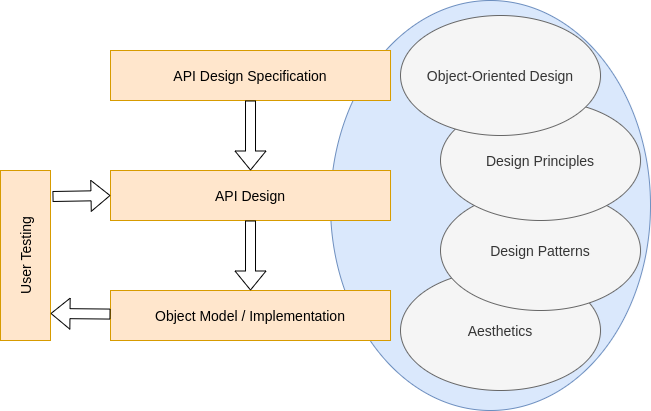
\includegraphics[scale=0.5]{images/api-design-process.png}
        \caption{Api design process}
    \end{figure}

    The API design specification consists a collection of the client-code and scenarios that guide the design of the interface. A scenario is a problem that needs to be solved by the API and the client-code is dream/pseudo code that should solve the problem presented.

    \subsection{API Design}

    The design of the interface is the interface’s structure. What areas of the interface can communicate, the file-architecture, which methods are needed and what each class should do. 

    \subsection{Implementation}

    Implementation is the actual code that is written. The details of the implementation should not leak out into the API. Design patterns and principles, and user-testing inform how the physical implementation develops.

    \subsection{User Testing}

    User tests are performed to gain a better understanding of how the user interacts with the APIs.Generally we would give the testers the updated Jar file containing the framework, a type reference documentation, and a set of scenarios to solve. These scenarios varied a lot from test to test. Since we emphasize scenario driven design, these problems are formed as scenarios that encapsulate a certain interaction with the API.  

    During user testing, there is an ongoing dialogue with the testers so we can guide them should they get stuck, or to answer general questions. At the end of the session, we run a quick discussion around their experience of the framework. This is where they express their thoughts and give feedback.

    The tests were done with groups 18, 40, and 5, as well as 5 other indivduals. In total, we ran 8 different user tests.


\section{Design Process/Results}

    \subsection{API Design Specification}


    \textbf{Process}

    All relevant scenarios produced are attached as an appendix.

    To develop the APIs, we employed Scenario-driven design. As a group, we discussed what we wanted these APIs to do. The requirements that developed from this process were:

    \begin{enumerate}
        \item To object-orient writing HTML and CSS.
        \item Have an almost one-to-one translation from HTML-tag and CSS-ruleset to java object.
        \item Write to file and give that file a .html or .css extension. 
    \end{enumerate}
    
    Based on these three main concepts for the API we created our initial scenarios for how this framework would be used. 
    The design and implementations of the APIs are slightly different as they were designed and implemented at different periods of the development process.

    \paragraph{Scenario 24}
    Make a website with a Form consisting of a field for e-mail, phone number, a text field and a submit button.

    This scenario hits on a few different aspects of the API. It requires a form class that has 3 different input-fields, and a button connected to it. We also need to put that form in a logical place in an html-file. This html-file also needs to contain a head with meta-data and necessary tags like a body, a header and a footer to be a webpage.

    \begin{shaded}
        \begin{lstlisting}
            WebPage myPage = new WebPage(); // initialize webpage

            ArrayList<InputField> listOfFields = new ArrayList();
            InputField emailField = new InputField(type: "email", name: "email");
            InputField phoneField = new InputField(type: "phone", name: "phone");
            TextField textField = new TextField(type: "text", name: "text");

            listOfFields.add(emailField);
            listOfFields.add(phoneField);
            listOfFields.add(textField);
            Form myForm = new Form(listOfFields);

            // generates html page in this order
            myPage.generateHeader(); // generate simple header
            myPage.append(myForm);
            myPage.generateFooter(); // generate simple footer
        \end{lstlisting}
    \end{shaded}

    Here we had usage of both high-level and low-level APIs. We could create simple one-to-one elements and we could automagically generate entire parts of a page. 

    \paragraph{Scenario 25}
    Make an article page with a title, an image and 5 paragraphs of text.

    Here the user needs to create the body, main, and other semantic containers for their website, but these tags do the same things. In addition, they need to be able to populate the containers with other html-tags.

    \begin{shaded}
        \begin{lstlisting}
            CreatePage thisPage = new CreatePage();
            int numbersOfParagraphs;
            String[numbersOfParagraphs] paragraphsText;
            Title titleName = new Title();
            Article articlePage = new Article();

            thisPage.add(titleName);
            thisPage.add(articalPage);
            GetImg img = new GetImg(String imgName);
            Paragraphs newParagraph = new Paragraphs()
            articlePage.add(img);
            articlePage.add(newParagraph(numbersOfParagraphs, paragraphsText));

        \end{lstlisting}
    \end{shaded}
    
    These scenarios created many questions about how the design should be. We started doing one-to-one translation between HTML-tags and java-objects, but now there were these containers that did not need to be their own classes.

    \paragraph{Scenario 14}
    Define a main grid for a website with 6 columns and 12 rows.
    
    For this scenario, the user needs to make a new grid object and define its columns and rows. The actual sizes are irellevant. 

    \begin{shaded}
        \begin{lstlisting}
            WebPage frontPage = new WebPage();
            Grid mainGrid = new Grid(
            new String[]{"1em", "1em", "1em", "1em", "1em", "1em"},
            new String[]{"1em", "1em", "1em", "1em", "1em", "1em","1em", "1em", "1em", "1em","1em", "1em"});
        \end{lstlisting}
    \end{shaded}

    This early psudo code for the CSS API shows how we initially wanted to pass CSS rules in the class constructors in the form of varargs. However, we realized this was not going to work as we could not tell which CSS property the constructor values would modify. A possible solution that we considered was to add multiple overloads to the constructos, however too many overloads could confuse developers and would not be a good practice for API design.

    \subsection{API Design}

    When designing the APIs in Silhouette, we started writing client-code to see what would work the best. We knew it was important to preserve the advantages of OOP, giving the user control by making objects and manipulating them in various ways. This meant that users have the ability to generate blocks of HTML quickly with the tools we already know from OOP.

    We designed the interface as a group, discussing how the classes would reflect the client-code. We separated the higher-level and lower-level aspects into their own packages, and decided that all html-elements would need to inherit from one superclass. The superclass then had all the base necessities of said element in a similar manner to the Factory method. However, there were many problems with this. Too many objects were being instantiated, no method-chaining, it acted clunky, and looked clunky, on top of being unreadable.

    This is where we were introduced to the Builder-pattern.

    \begin{figure}[H]
        \centering
        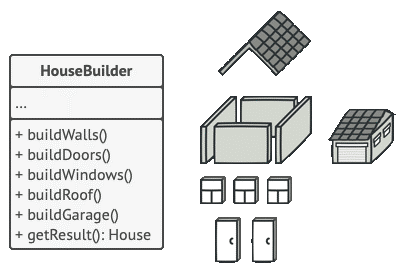
\includegraphics[scale=0.5]{images/builderPattern.png}
        \caption{Builder Pattern Visualized}
    \end{figure}
    
    Later on once we got some feedback from other groups we came across another problem. Users expected to be able to chain multiple methods after another. But that was just not possible with how we originally structured our methods and classes, that's where builder pattern comes in. Builder pattern aided the framework in two areas: One, it served as a tool to hide the backend-implementation from the user, and two, it allowed for method-chaining which was exactly what we needed.

    Builder pattern helped to account for all the different options when writing HTML and CSS. The pattern creates a structure in the code that consists of building components and appending them to each other. It organises the process of creating objects into steps, so one can make the same object look very different depending on how it was put together. Using a director on the builders allows for even more abstraction that we could use to develop a base for a high-level API.

    This design pattern allows for the making of immutable objects and method chaining, and it made the code a lot more readable, though still somewhat repetitive.
    
    Now we needed to separate functionality. Which classes belonged, and what needed to be extracted. Following the Single Responsibility Principle, each class should have one and only one responsibility. In most cases we have tried to follow this as best we could. The one-to-one mapping that we initially built the API around was due to this principle, though deprecated or exceedingly similar HTML-elements were left out of the design and implementation, some due to time constraints, and some because they were better to combine, such as all page section-tags( $<$div$>$, $<$main$>$, etc.). The HTML-class currently has too many responsibilities and breaks with this principle, due to the initialize()-method, which means the html-class currently both represents an html-tag and the an html file. The compiling and writing to file should happen in its own class like it does in the Framework’s CSS API.

    Abstraction to interfaces within the API allows for different implementations of the same method in multiple classes. Sticking with the interface segregation principle, we tried to ensure that these interfaces would only have a few specific tasks. 

    \begin{figure}[H]
        \centering
        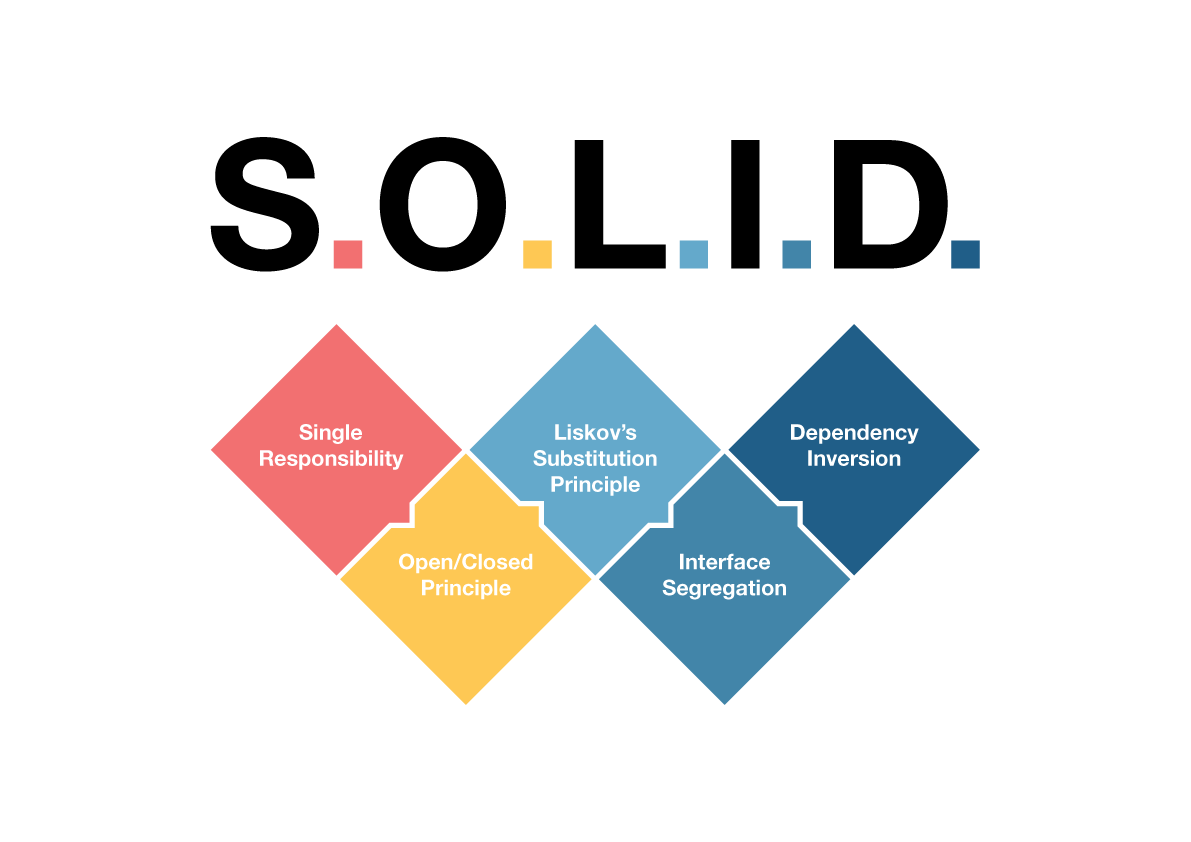
\includegraphics[scale=0.5]{images/solidGraphic.png}
        \caption{SOLID Principles of Software Design}
    \end{figure}

    \subsection{Implementation}

    Most non-abstract or static classes received their own internal static Builder class during the initial implementation, however some classes did not, like the Paragraph and Heading classes as they could be considered very small, and are used with high frequency. Though it unnecessary to implement the pattern here as well, due to user-test feedback, we decided to after all, since the change in pattern broke with the development flow. This led to the implementation of builder-classes for every class in the API that should be instantiated.
    
    The top-level builder has been abstracted into its own interface. This interface is then implemented in each of the internal builder-classes. Even though a lot of very different looking objects are being created, both the higher- and lower-level components of the API should depend on the same abstraction, so there is some achieved dependency inversion, though implementation is not complete.

    The biggest problem with the implementation of the Builder-pattern, and attempting to apply these principles, is that the builder pattern usually doubles the amount of code necessary, and using correct abstractions can be very difficult.

    Implementation was done in various stages as we had many ideas for how we wanted the resulting framework to behave. After a lot of discussion with the group, we began writing client-code to help us visualize the API to get better ideas on how we got incorperate the implementation. After several supervisions with the lectruer, we were advised to use a builder-pattern, which works wonders for the type of tasks we want to do, however it makes implementing a bit of a chore, as this means usually our source-code will double. Getting to understand how this pattern works was not easy, since as we were writing our API-code we did not have a full understanding of the structure of method-calls/chaining, nor how to really instantiate these objects. This led to some early errors like giving each builder-class a specific name, and not implementing it correctly.


    Lastly, we needed to form a system to generate the actual file. The big idea was to make some sort of compiler that puts strings together to make the necessary web files. It later became apparent that we needed one compiler for each API, as the logic and syntax are wastly different. As it stands, the compilers will either read html and css in the form of Strings, or plain java old objects (POJOs). Then once the user is done defining their pages and stylings, they will inform the respective compiler to perform a compile and generate the web files. If these files already exist, the compiler should just overwrite them to apply the new changes.


    \subsection{User Testing}

    User testing started after a month of developing the first iteration of the API. At this point the low-level HTML API felt almost complete, however the high-level-, and CSS-APIs were bare minimum. The implementation was not ready and the APIs consisted of plain old java objects. It was therefore important know if the names and overall use made sense, and if there were any major flaws that we could improve upon.

    After the testers solved the scenarios using our framework, we would have a quick discussion with them about their thoughts and opinions. As they expressed their views on the framework, we would take notes and often ask some follow-up questions. At the end of the session we would ask some general questions to see how their views compared with other testers. This would help us see how the changes affected the framework, as other testers had different opinions.

    After the session with the testers, we would have a discussion with eachother about the feedback we got from the user testing. Since each group member had their own focus areas in the development, this would help a lot to get insight on the next big changes we were going to implement. 

        \subsubsection{Frist user testing session (Silhouette-HTML v.2)}

        Right after they had tested our framework and completed the setup, we asked them to give their initial reaction and opinion. They said, “It was pretty good once we got the hang of the class names” which was a relief to hear. It seemed to us that they found the APIs to be intuitive, as they quickly grew familiar with the main classes. We then followed up with a few questions regarding their experience, and they told us they could easily expand further on their website with enough practice.

        \subsubsection{Second user testing session (Silhouette-HTML v.2)}

        This user testing toke more time that what was needed, if it wasn’t for an error from our side in the code structure. When we found out what the error was and the confusion was over, it was back to the user testing, but the person that was testing the program was stuck and didn’t understand how to start and/or what to write (defining the html-object). After some time we gave the user a push in the right and the user started to type/write like it was natural for them or as the hade used our framework before.

        \subsubsection{Third user testing session (Silhouette-HTML v.2)}

        In this user testing the tester was tested in a different way, where the tester received minimal help and mostly through think and some fiddling on their own, because of the users higher understating to code structure and language.

        The user managed the first part of the task easily (due to the naming of classes and method names) but began to strive on the second task. The user was supposed to create a new object called "Container", but started working on the method calls instead (because it seemed most natural to them) and had to ask for help and then came the next problem... what are Builders.

        After some explanation it came naturally and the rest of the second task was then over and the user was on their owe, with a little hint here and there. The user could see the logic but felt that it lacked a flow in the structure and believed that getting in to "Silhouette" for a new user is not easy without a manual or help from someone.
        
        \subsubsection{Fourth user testing session (Silhouette-HTML v.3)}

        Fourth testing was done in a group context, where one of them wrote and the others watched and tried to understand "Silhouette" (I also had to describe how Builders works).

        It started the same with this group as it was done with the other user testing section, but since one of the user was looking through the library and was reading the methods that had a similar name as in HTML, one tester got an idea what to write and they managed to complete this task. And they applied the same tactic to the next tasks, and they managed the whole user testing with a few hints. 

        \subsubsection{Fifth user testing session (Silhouette-HTML v.3)}

        The fifth test was carried out by a student with a good knowledge of java and HTML, who wanted to learn the framework (“Silhouette”) from top to bottom. The user spent 1 hour and 30 min doing the task (without help) and gained insight into how "Silhouette" HTML.BaseComponents.* (file's) worked. This user was more interested in the "Silhouette" library and gave some feedback about that the structure is easy to understand, but there was a lack of comment (you can't read comments for a jar file) on what the methods do/did, etc. and that the end result might affect a user “Silhouette’s code” and meant that “it’s too hard-coded” when a user is done with it.

        \subsubsection{Last user test}

        For the last user test we tested with a student who previously had the same framework course, and who was very familiar with builder pattern and API design. The session took about three hours, and we tested both the HTML API and the CSS API. We sent the Jar file of the newest version of the framework to the tester, a type reference documentation, and some scenarios to solve with the framework.

        \textbf{Make a new HTML page. Set a custom title, and set the charset meta tag to "UTF-8"}

        \textbf{Scenario 17}

        For scenario 2, the user were instructed to make a body element and add it to the page. At first, it wasn't very obvious for the user to use the Container object to build the body element, as it is passed through the parameter. After some explanation, the user understood why we had done it that way, but still felt like it was not as intuitive. The user commented that it would be much better to just separate the most important layout elements into their own class, though this was already discussed within the group at the beginning of the project. Having a class for each element comes with two major issues. Firstly, if we would simply make a class for each element, there would be too many classes to keep track of. Secondly, how would we decide which element needed their own class? Because of this we decided to keep it as originally planned.

        \textbf{Scenario 18}

        Here the user found it confusing that there were two ways of adding a heading to a container element. While the intended solution was to make a Heading object, the user opted for the addHeading method inside ContainerElement.

        \begin{shaded}
            Making a Heading object

            \begin{lstlisting}
                Heading myHeading = new Heading.Builder()
                        .setLevel("h1")
                        .setText("My heading")
                        .build();
            \end{lstlisting}

            Using the addHeading method inside ContainerElement

            \begin{lstlisting}
                Container div = new Container.Builder()
                        .addHeading(1, "My heading")
                        .build();
            \end{lstlisting}
        \end{shaded}

        Initially, this was done to give users more options when declaring the markup. However, this proved to be more confusing then helpful, so we decided to remove this additional method.

        \textbf{Scenario 19}

        Right off the bat, his impression was that we had over-used the builder pattern, to the point where it becomes unecessarily complicated. For example, the user explained how it was unecessary to use builder pattern for the Paragraph class, as the paragraph should only take one argument in the constructor anyway. The user suggested that it would be better to simply pass the text to the constructor.

        \begin{shaded}
            With builder pattern

            \begin{lstlisting}
                Paragraph p = new Paragraph.Builder()
                        .setText("Hello, World!")
                        .build();
            \end{lstlisting}

            His suggestion

            \begin{lstlisting}
                Paragraph p = new Paragraph("Hello, World!");
            \end{lstlisting}
        \end{shaded}

        His suggestion was not bad, but since we wanted to follow the same convention for every class, we felt it was better to leave it as be with the builder pattern. That way, there is not confusion whether it uses the builder or not. We also find the parameters more clearer with builder pattern, as it explicitly shows it in the method name.

        \textbf{Scenario 20}
        
        At first the user was not fond of using enums when adding a new rule to the rule set, but quickly the user grew the habit of using them. The user commented that it felt unecessary at first, and that they would rather type in the propeties and values as a string. But after explaining why we use them (which is to make sure the user does not pass inn misspellings), the user understood and agreed that it was a good solution.

        \textbf{Scenario 21}

        
                

        To finish off the session, we asked the user for some general questions about the framwork. Firslty, we asked the user about what they thought about the name "Silhouette", and if they found it intruiging and informative. To this, the user told us that the name is as ambiguous as most other names out there. They stressed, that it does not necessarily mean it is bad, but it did not give them any idea of what the framework did. At this point, we have become very fond of the name, but it is always nice to get feedback.

        We also asked the user found the framework to be difficult to use. To this the user responded that builder pattern greatly increases the amount of code needed to generate a website, so in this case it would be faster to write it in standard HTML and CSS. We agree to this, wowever, we are still of the belief that the OOP aspects and the additional make up for it. Another issue for the user was the quality of the type reference documentation, as it often failed to give the user a good idea of what each class represented.

\section{Resulting Framework}

    See JavaDoc for project-structure and source code.

    \paragraph{Scenario 24}
    Method-chaining through the builder-pattern allows for the creation of an entire HTML-file in a single line of code.

    \begin{shaded}
        Creating a paragraph and adding it to a div
        \begin{lstlisting}
        new HTML.Builder()
            .addElements(new Form.Builder(new FieldSet.Builder()
                .setInputs(
                    new Input.Builder()
                        .setLabel("email")
                        .setId("email")
                        .setName("email").build(),
                        new Input.Builder()
                        .setLabel("phone")
                        .setType("tel")
                        .setId("phone")
                        .setName("phone").build()
                        new Input.Builder()
                        .setLabel("name")
                        .setId("fullname")
                        .setName("name").build(),
                        new Input.Builder()
                        .setType("submit")
                        .setValue("Submit").build())
                    .build())
                .setAction("/dest.php")
                .setMethod("get")
                .build())
            .build()
            .initialize();
        \end{lstlisting}
    \end{shaded}

    Whilst not necessarily the most straight forward way of coding, the style is easy to read, in effect making the barrier of entry, for most programmers, low.

    \paragraph{Scenario 14}
    Define a main grid for a website with 6 columns and 12 rows.

    \begin{shaded}
        \begin{lstlisting}
            Grid myGrid = new Grid.Builder()
                .addRule(Property.GRID_TEMPLATE_COLUMNS,
                    "1em 1em 1em 1em 1em 1em")
                .addRule(Property.GRID_TEMPLATE_ROWS,
                    "1em 1em 1em 1em 1em 1em 1em 1em 1em 1em 1em 1em")
                .build();
        \end{lstlisting}
    \end{shaded}

    This client code shows the newest style sheet API and the clarity of using the builder pattern. Builder pattern makes the code a lot more readable and makes it possible to dynamically change the property and value parameters in the chained methods. 

    \subsection{Patterns, principles and user feedback}

    The framework consists of two low-level APIs that cover their own aspect of web-development. Both are object-oriented conversions of declarative languages; CSS and HTML. The designs of the two APIs are drastically different as the one-to-one conversion for the HTML API was slow and clunky. This process was very time-consuming, and, due to the mapping, the pattern led to bloating of the source code. This was unfortunately an issue we never were able to address for this API, as we had already invested too much time in its implementation at this point.

    The stronger aspect of this implementation is SRP. All classes have only one responsibility, except the HTML-class. This means that changing something in a class will not affect the rest of the API, just the parts dependent upon it. Avoiding random dependencies within the API, keeping the code DRY and creating logical dependency inversion abstractions was a large part of understanding how to develop the framework.

    The CSS API has a more cohesive implementation. This API does a lot more with a lot less code. Though this API requires a greater understanding of design and development than the HTML API does, it too was initially based on the factory method of design. The abstract class was implemented, and its children look like it with variations. This is a much more correct application of the builder-pattern, as the objects created are essentially the same, with small variations, unlike the HTML API which uses the pattern to create very different objects using the same process.
    The use of internal Builder classes was an early decision that was made due to a lack of knowledge about the application of the pattern. Though no one way is correct, extracting these inner classes into their own package, and referencing their respective products would be a lot cleaner, and require slightly less code.

    What informed the resulting framework and its functionality was user-testing and related feedback-discussions, this is where the process of Scenario-driven design shines. Initially the builder-classes behaved very differently from each other. Some builder-constructors would have parameters and others not, set-methods would allow for different types in their parameters and not just strings, or the internal objects, as was the most used methodology throughout the API. Through user-testing we discovered these differences, how they changed way the testers applied the coding pattern, and experienced how they affected the development-process of others.

    In the end, all classes in the HTML API have the same behaviour, making it consistent and intuitive in use. The CSS API implementation took inspiration from the HTML API, however opting for an inheritance based pattern instead.

\section{Discussion}

    \subsection{User testing tactics}
    One tactic we had was to find people with knowledge in Java and in HTML and/or Css who can test "Silhouette", without providing training in one of the coding languages to the user, although that we had to teach the different users how Builders works.

    And after some user testing, we got a feel for what worked and not in the user testing, and we agreed to create a task/test to test the different users to see what the difference between one user and the other user and compare the different users in the same user testing, but since we didn't have that many user testings, it ends up being something that we couldn’t tested properly or not at all, but the focus was on the visual code structure that the user wrote and what they thought about it, if they understood what they wrote, what do they think about the logical structure of the code they have written and smaller fixes that "Silhouette" needed. for example, Heading took in an int to create the "hx-tag" and people wondered why not use a String so that you can write h1 to define the header type, instead of a number to make it less confusing.

    \subsection{Project size and time frame}
    Our biggest problem is that we have created a large framework (compare to other groups) and there is a lot that has had to be added to this project, if we are to follow our project plan for how "Silhouette" should work. Much of our time was put into the other subjects/lines we had and created poor work distribution in this subject. And when we were working on the project, a lot of the work was put into creating code that was best for the user (the visual code structure and simplifying the code) and that's one of the reasons why we chose to use the Builders method.

    When reading through the code and structure of Silhouette, it will be clear that the low-level section is API that has received the most attention and that there multiple classes still needs implementation. 

    \subsection{Working with the different group members}

    It started with 2 months of hard work and 2 months on and off and started working on the frameworks again approx. 1 week before the submission of project.

    At first everything worked well, everyone had the same idea of what we were going to make and what it would look like. We did "First Delivery" together and had many good discussions about what can work in our project and not. Everything we had created was sent in for feedback on the ideas about the build-up of "Silhouette". After many meetings and work sessions, "Silhouette" was in v.1 (or a prototype/idea), but it's not ready for testing yet. We knew about some errors and things that needed to be improved before it was ready for testing, but all the methods calls were in place. So you could write the "Silhouette" code, but it did't do anything.

    Around this time, one of the group members started struggling a bit (illness and stress), but the others group members told that person, to take it easy for a while and we'll fix this, so they got more workload and thats not really good for the group moral. They work on the project and deliver "Second Delivery" without this members help and around this time we/they start working on each part of the project, where one member works with the HTML section and another member works with the CSS section and "Silhouette" was approaches v.2 and we started using something called Builders. Around this time "Silhouette" is starting to become little bit complicated. One of the reason we did not touched each other's work area, is so that we don't make any merge conflict and messing up the code structure for each other and create more workload.

    Then that group member comes back but had a new problem now. This member barely has time for all the subjects because of another group assignment that this member has and this member considering leaving a subject in order to focus on frameworks, but the group supports this member by saying “we will fix this and don't drop out of any subjects you have” and it's around this time the 2 months of the break (on off working) comes and they're started doing the "Third Delivery" without this member again.

    Around 1 month before delivering the group assignment this member is back for more work, but since the others the group members have a lot to do in one of their subject (we have different fields of study and that didn't create that much problems for us after all), the frameworks was put on hold for a little bit more. So, this member began working on some user testing to not waste time, but after some trials and errors the member had some idea for how to optimize the user testing. When the other group member came back, they work hard for a few days and "Silhouette" is in v.3. Because of the changes for v.2 to v.3 all the code structure are Builders and the user testing feels more naturally for the user and that is what we wanted.

\section{References}

[1]: Chevalier-Boisvert, M. (2015). \textit{The Problem with HTML}. \\ Retrieved from https://pointersgonewild.com/2015/04/16/the-problem-with-html/

\end{document}